\section{Exemplary Memory Access Visualization Tools}\label{sec:works}

This section examines several prominent works dedicated to visualizing memory movements and accesses. Each tool will be discussed in terms of its data gathering methods, visualization techniques, and demonstrated results. We will then contrast these tools, highlighting their strengths and weaknesses.

\begin{figure*}
	\begin{subfigure}[c]{.48\linewidth}
		\centering
		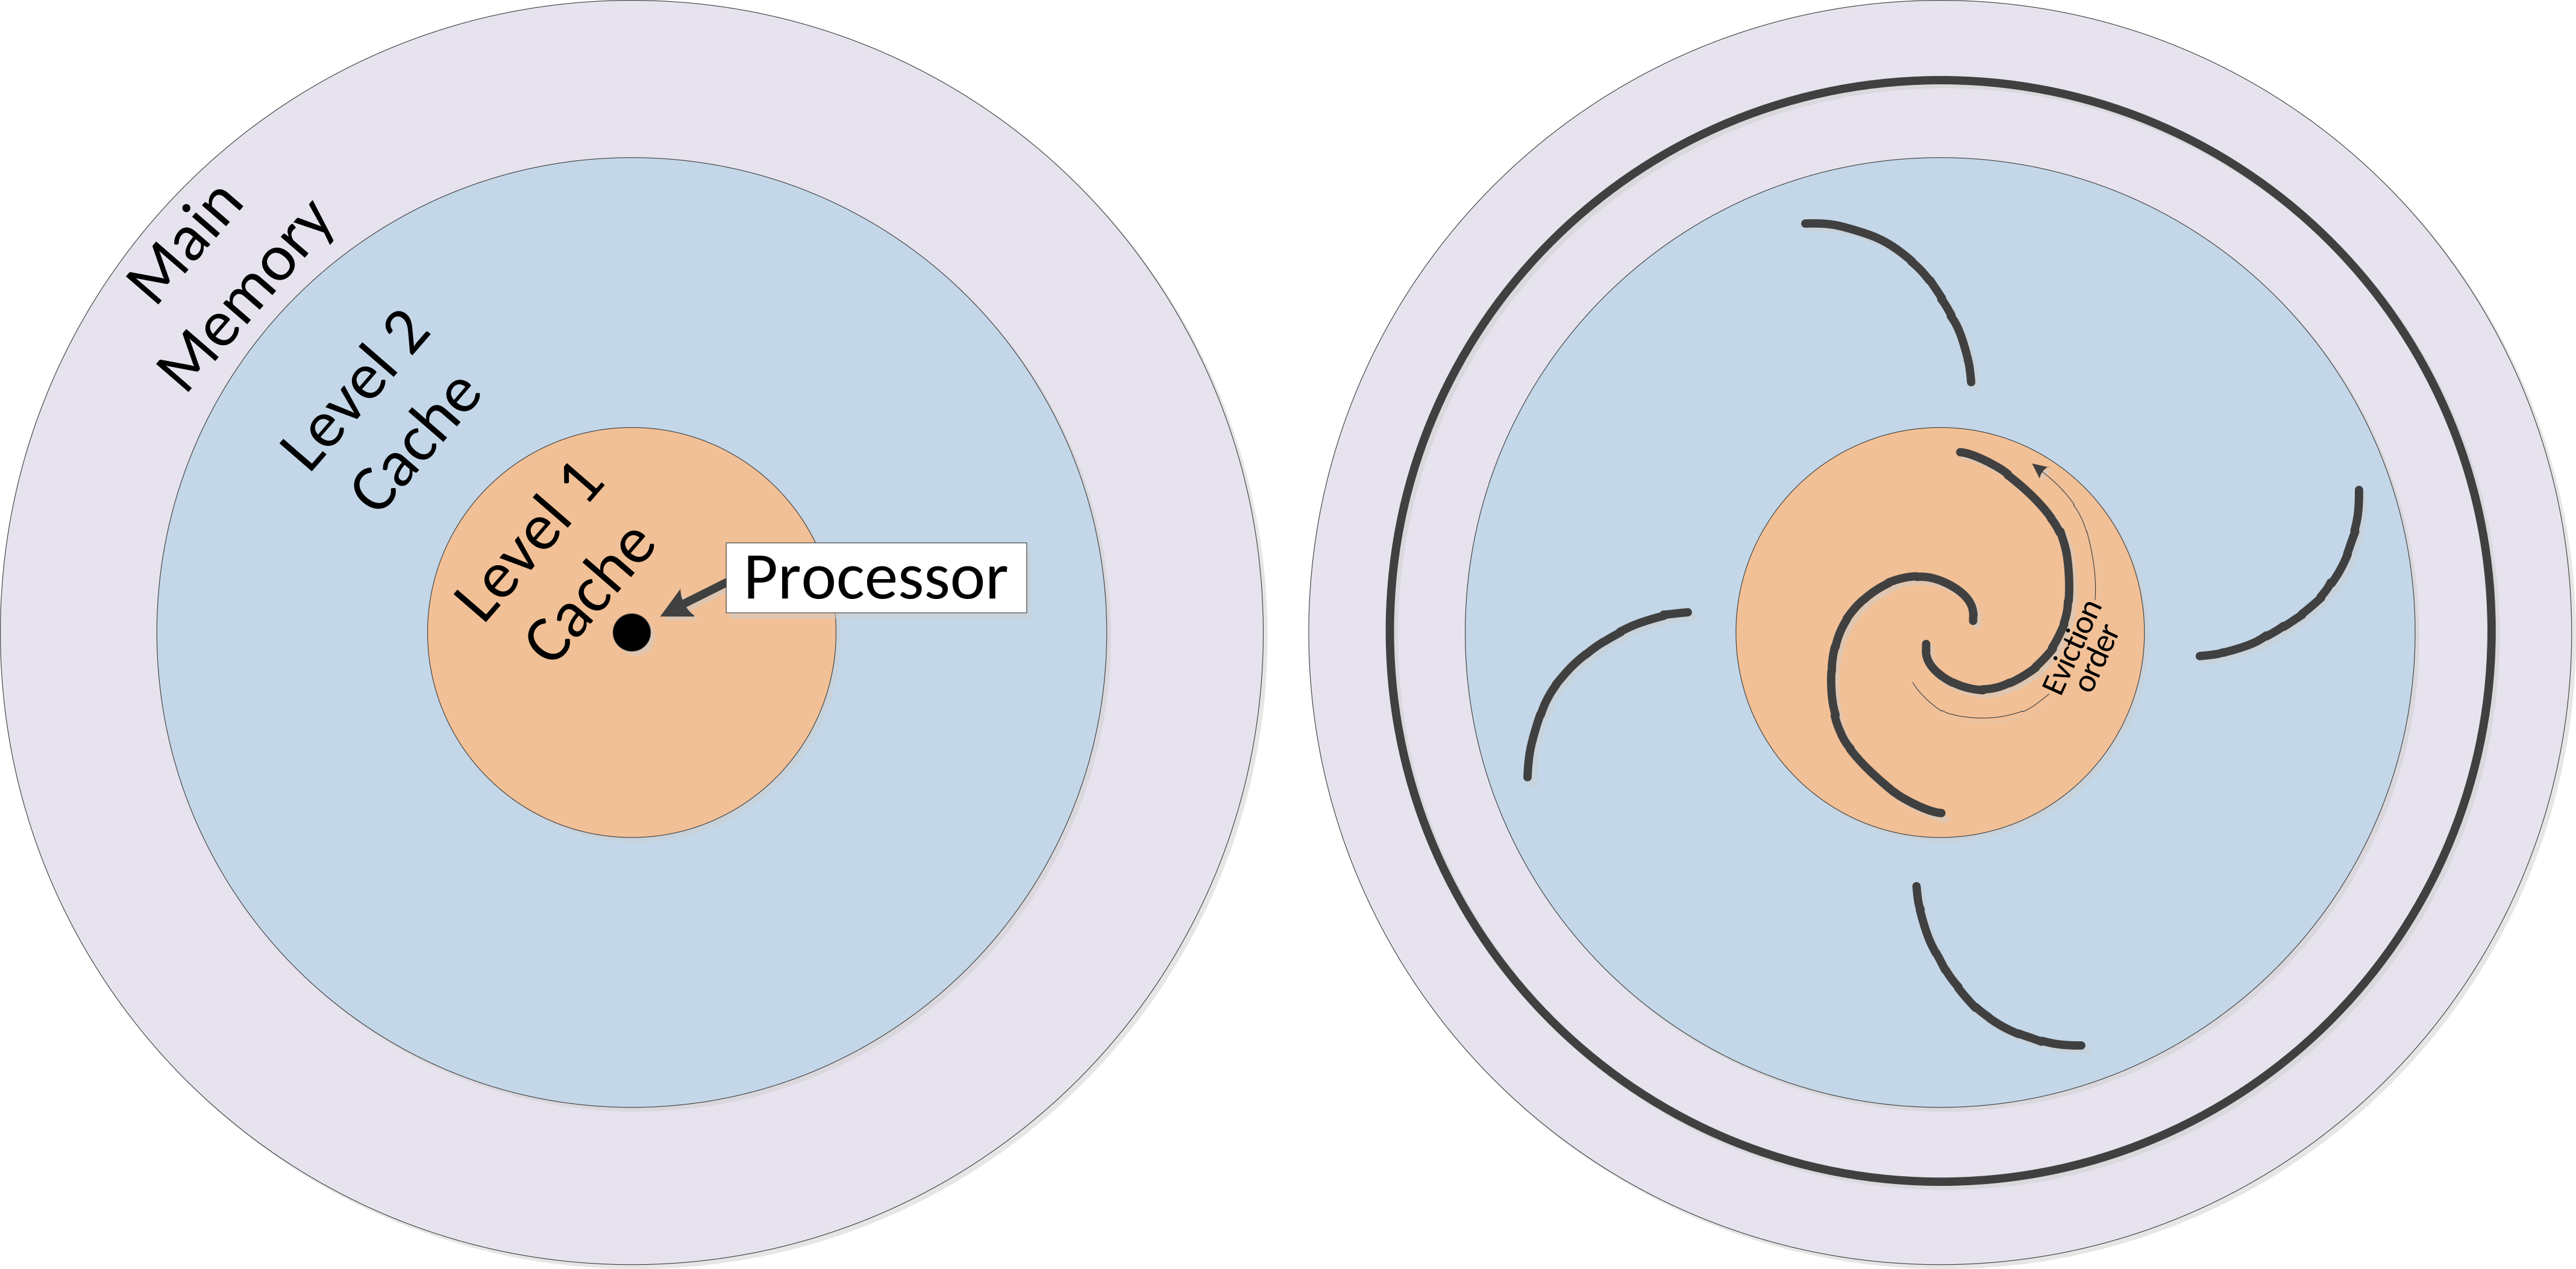
\includegraphics[width=\linewidth]{pictures/abstract_explanation.png}
	\end{subfigure}
	\begin{subfigure}[c]{.24\linewidth}
		\centering
		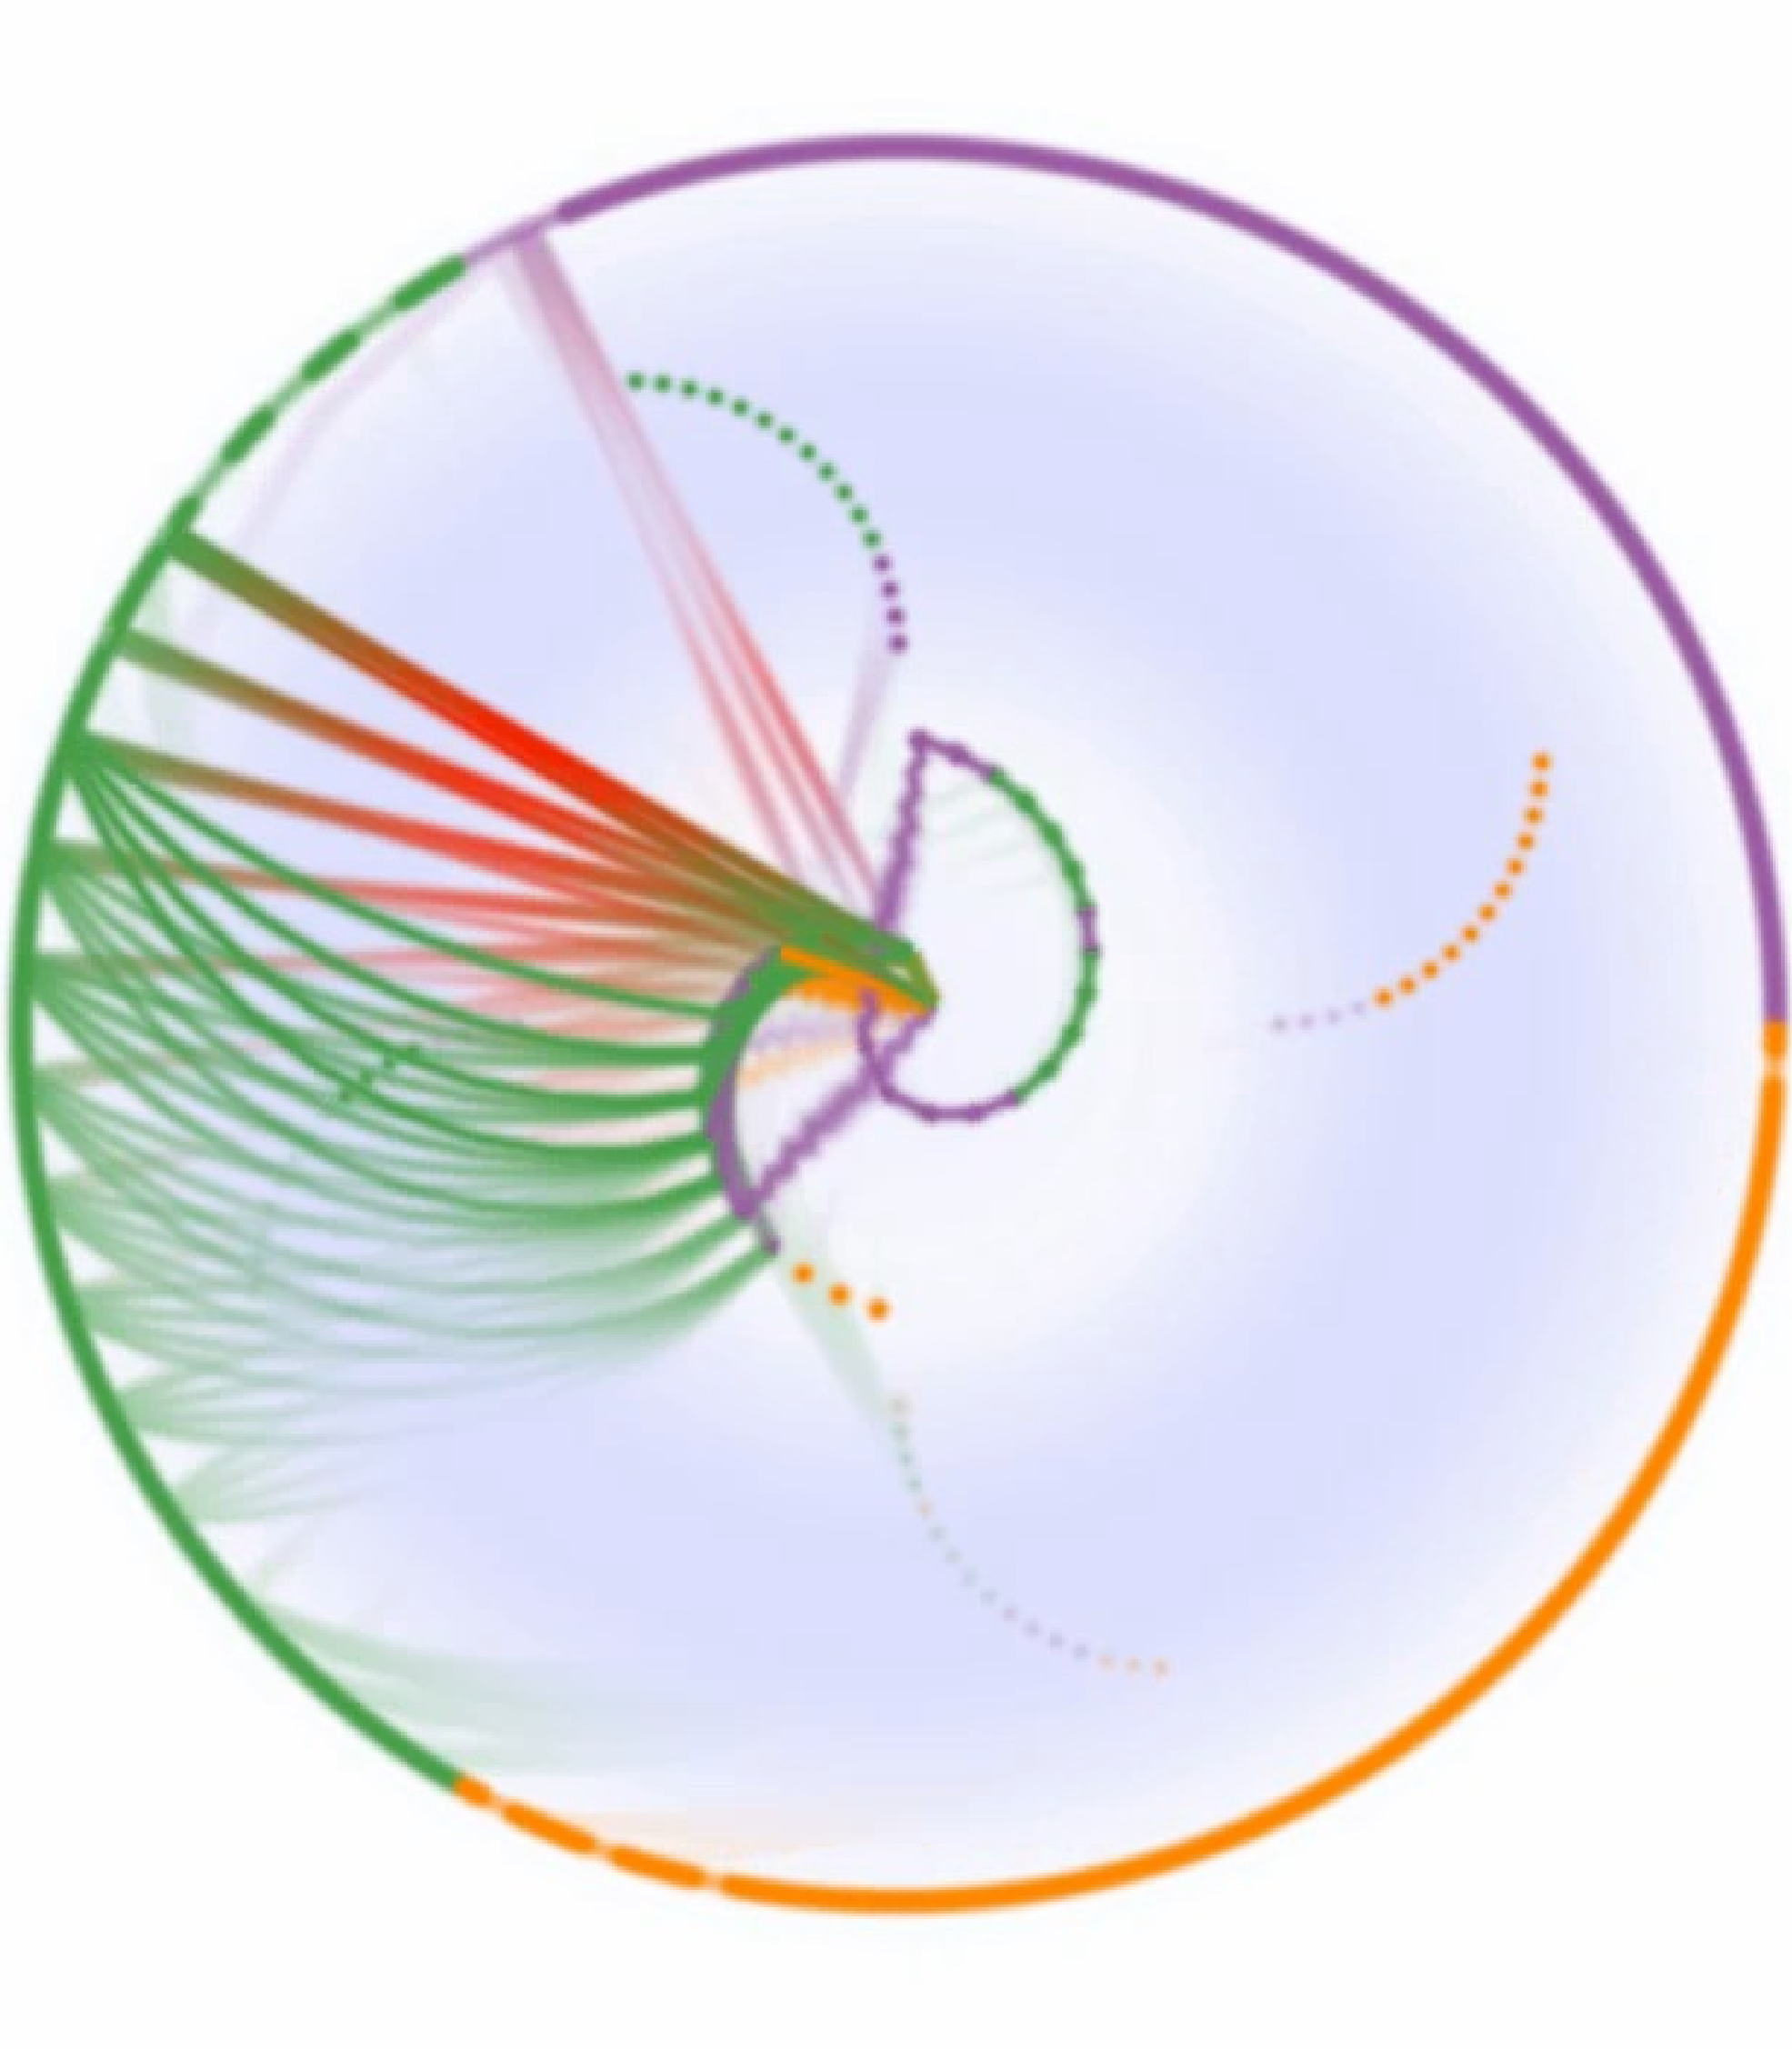
\includegraphics[width=\linewidth]{pictures/abstract_standard.png}
	\end{subfigure}
	\begin{subfigure}[c]{.24\linewidth}
		\centering
		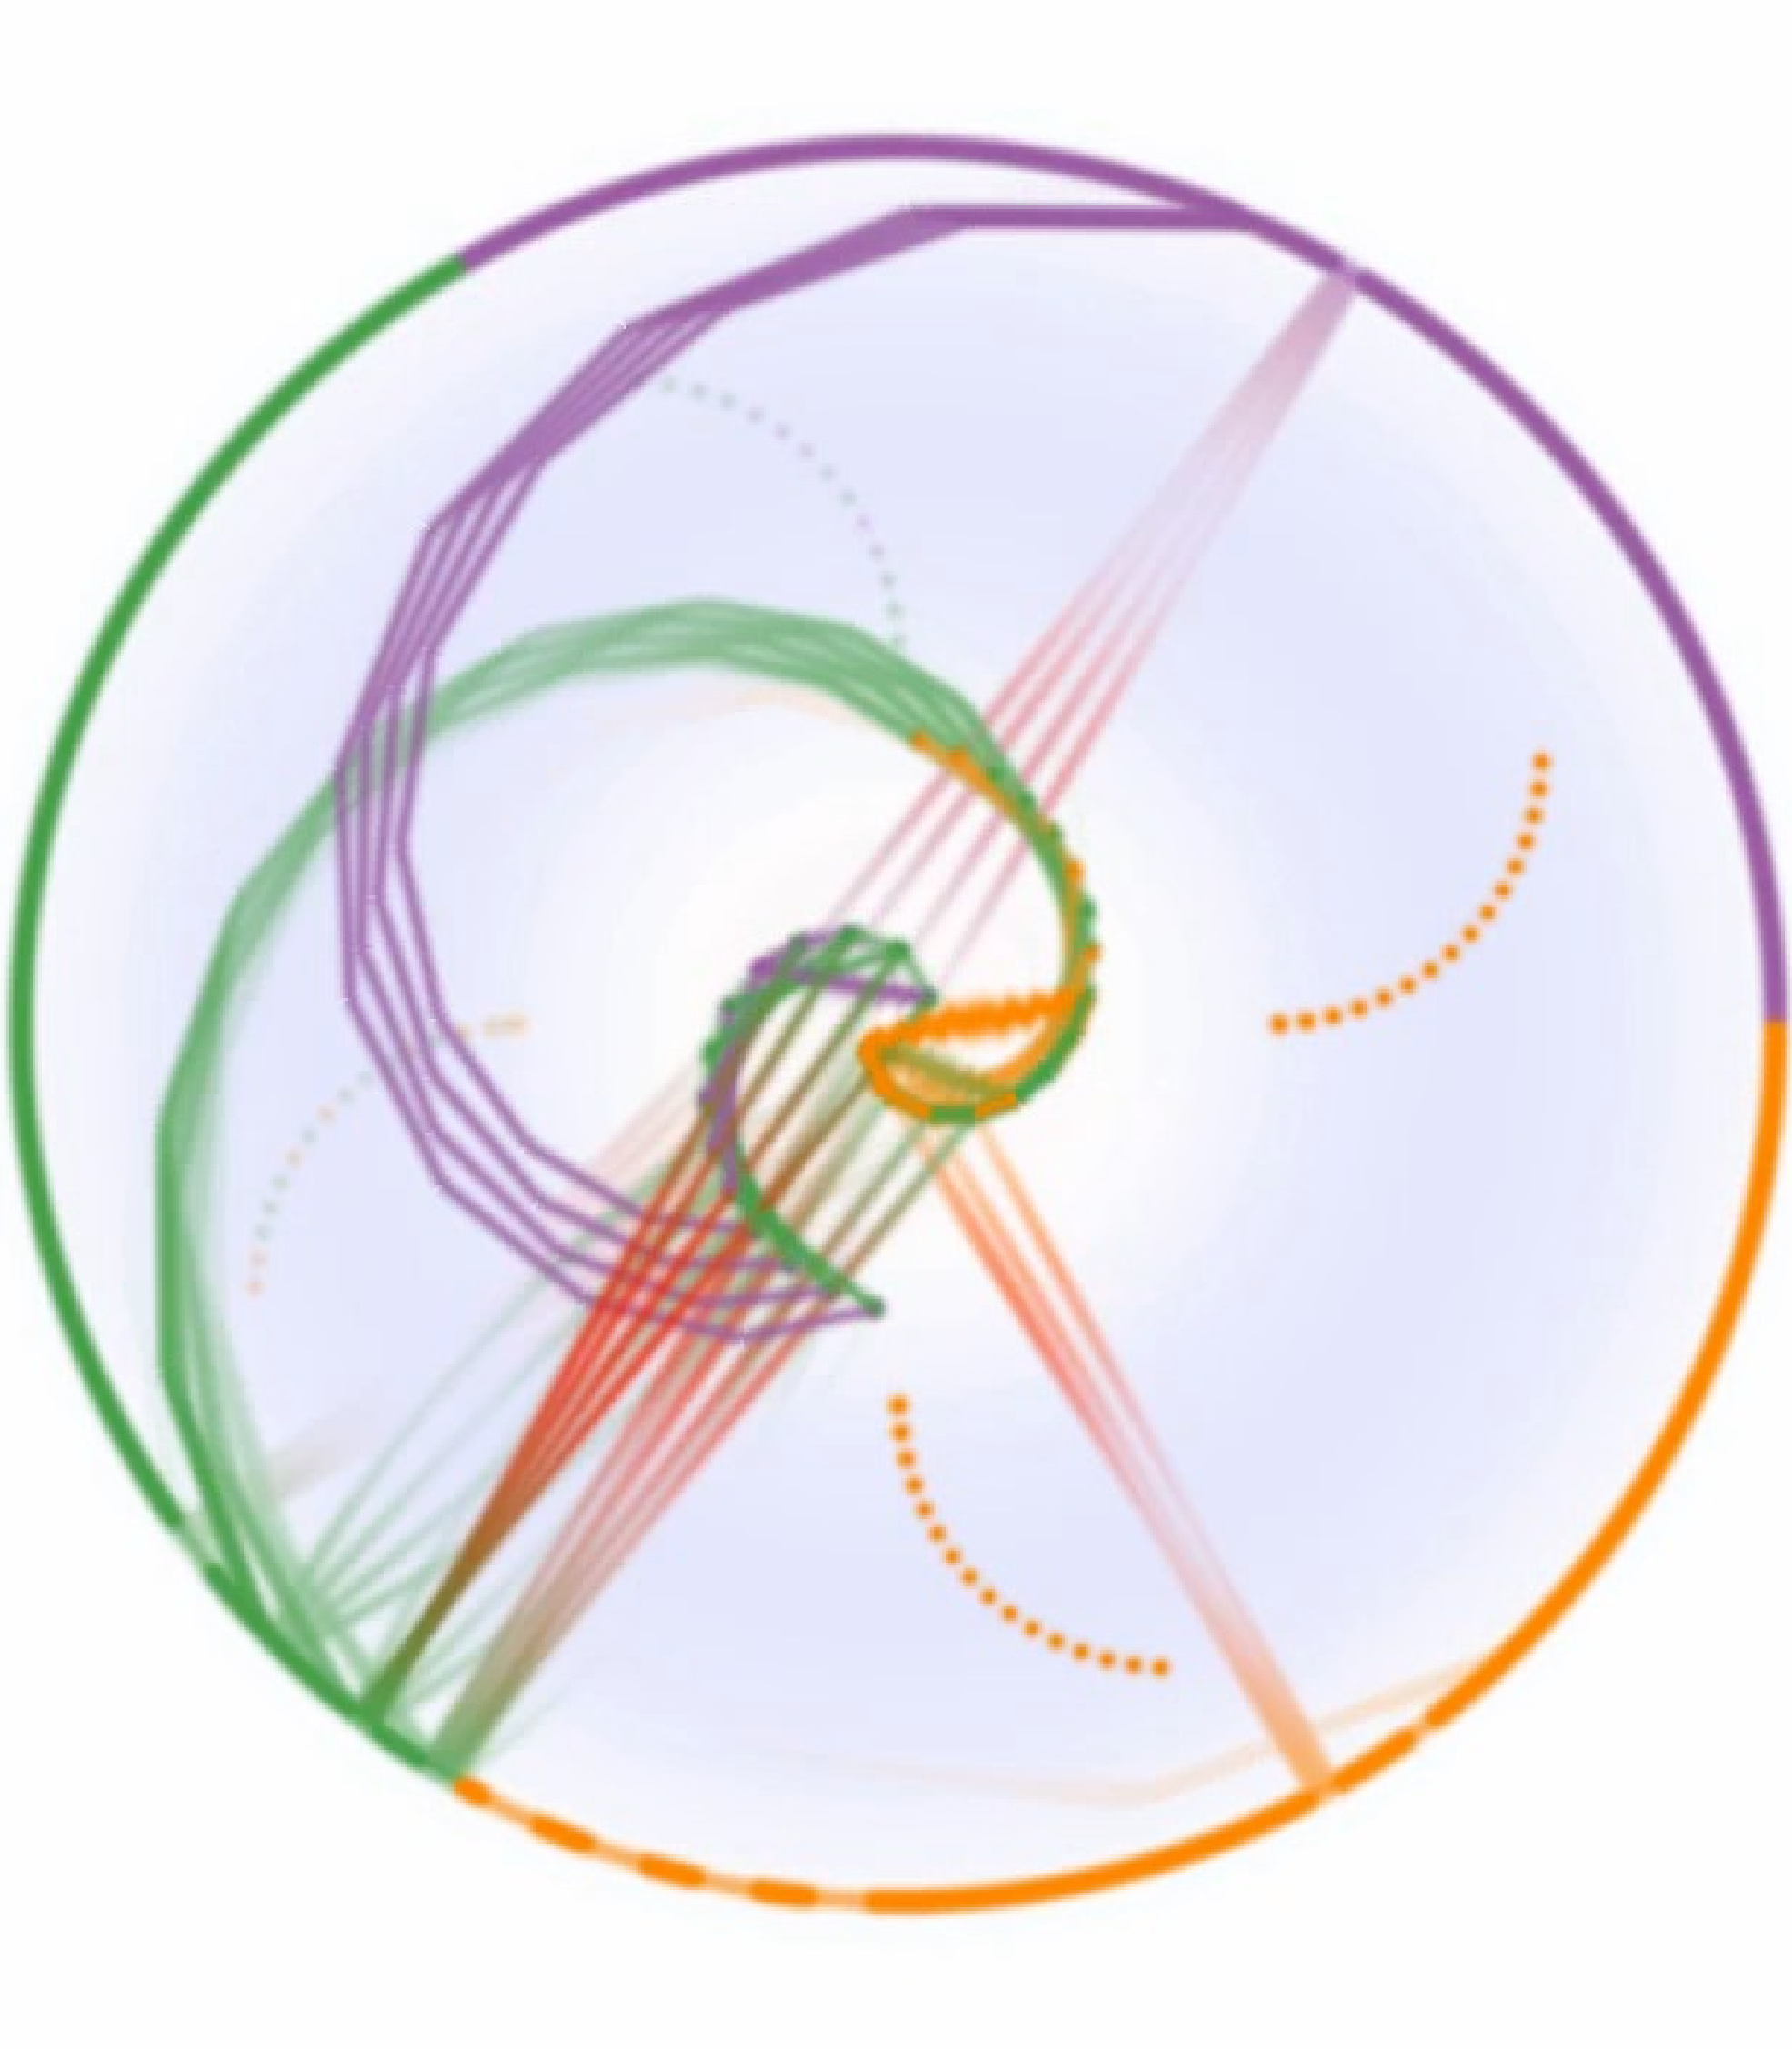
\includegraphics[width=\linewidth]{pictures/abstract_optimized.png}
	\end{subfigure}
	\caption{Left: Radial design used in \cite{choudhury2011abstract}. Glyphs arrange themselves into groupings indicating storage on the same cache, with data closer to the boundaries between the levels more likely to be evicted. Right: A comparison of a standard $16 \times 16$ matrix multiplication and an optimized version using $4 \times 4$ blocking. The standard version shows poor data reuse for two of the three matrices \cite{choudhury2011abstract}.}
	\label{fig:abstract_cache}
\end{figure*}

\subsection{MemAxes: Visualization and Analytics for Characterizing Complex Memory Performance Behaviors}\label{sec:memaxes}
The tool \texttt{MemAxes}, developed by Giménez et al. \cite{gimenez2017memaxes}, utilizes dynamic analysis (Section \ref{sec:dynamic_analysis}) to generate an event log of memory accesses. Each logged event incorporates contextual information, facilitating a link back to the source code and recording the memory hierarchy depth at which the memory access occurred. This feature allows for the identification of problematic code lines, similar to \texttt{HPCToolkit} \cite{adhianto2010hpctoolkit}, as illustrated in Figure \ref{fig:coarse}. Recording the resolution depth of memory access enables the determination of resource utilization across each memory module and the quantification of physical data movements between them. This information is then visualized using a radial design of the hardware topology, as seen in Figure \ref{fig:memaxes_cache}. \texttt{MemAxes} also supports the display of additional attributes such as access times, latencies, and memory addresses through histograms.

In practical applications, \texttt{MemAxes} has been employed successfully to detect and mitigate performance bottlenecks, even without prior knowledge of the application's source code \cite{gimenez2017memaxes}. Performance engineers can, for instance, identify large load imbalances or significant spikes in access times, and use these insights to hypothesize the cause of a performance bottleneck. This hypothesis can then be explored further through the backlink to the source code. This approach demonstrates that low-level visual aids are not necessary for optimizing data locality in an unfamiliar program.

\subsection{Abstract Visualization of Runtime Memory Behavior}\label{sec:abstract}

Choudhury et al. \cite{choudhury2011abstract} offer a unique perspective on runtime memory behavior through their visualization tool, conceptually different from \texttt{MemAxes}. Their approach involves dynamic analysis to chronicle an event log of memory accesses during runtime (Section \ref{sec:dynamic_analysis}), which then feeds a cache simulator (Section \ref{sec:simulation}). The output is a series of radial visualizations, exemplified in Figure \ref{fig:abstract_cache}, which are generated throughout the program's execution, forming an animation of evolving data movements within the memory hierarchy.

The visualization in Figure \ref{fig:abstract_cache} uses a concentric layout to demonstrate memory usage patterns. Glyphs, symbolizing memory locations, navigate across layers representing main memory and different cache levels. Movements towards the center imply recent references, while those towards the periphery indicate aging or eviction. Performance issues, such as inefficient memory usage or frequent evictions, are suggested by rapid, large-distance glyph movements. Conversely, slow in-layer movement indicates high cache hits, signaling efficient memory utilization \cite{choudhury2011abstract}.

Choudhury et al. argue that this dynamic approach is more intuitive than static visualizations, such as those provided by \texttt{MemAxes}, as it presents an overview of large-scale memory access and caching behavior. However, its granularity is insufficient for targeted bottleneck resolution, given that the visualizations lack linkage to specific contextual information such as precise addresses or lines of code.

\subsection{Boosting Performance Optimization with Interactive Data Movement Visualization}\label{sec:boosting}
The tool developed by Schaad et al. \cite{schaad2021boosting,schaad2022boosting} enables two-tier program analysis:

At the global level, static analysis (Section \ref{sec:static_analysis}) is used to compile the program source code into an SDFG graph, providing an overview as shown in Figure \ref{fig:coarse}. This graph, with its color-customizable nodes and edges, aids in identifying problematic program sections, especially when utilizing the automatic node and edge collapsing feature for easy zooming.

For in-depth analysis of data locality and reuse behavior, the tool uses cache simulation (Section \ref{sec:simulation}) to offer detailed views of specific program segments, as depicted in Figure \ref{fig:boosting_cache}.

The authors successfully employed this tool to significantly optimize two applications. After pinpointing problem areas in the global view, the engineers utilized the local view for a thorough investigation and subsequent optimization of these areas.

\subsection{Comparison}\label{sec:comparison}
Among the three tools, the animation provided by Choudhury et al. \cite{choudhury2011abstract} offers the most intuitive understanding of large-scale memory access and caching behavior. However, comprehensive program optimization requires contextual information about inefficient memory access locations, which is supplied by \texttt{MemAxes} \cite{gimenez2017memaxes} and the tool by Schaad et al. \cite{schaad2021boosting}. Of all three, Schaad et al.'s tool provides the most detailed low-level visualizations. The tool's ability to depict the influence of data layout on the cache hit ratio proves invaluable for optimizing data locality. However, the tool's reliance on cache simulation necessitates consideration of parameterization, as discussed in Section \ref{sec:simulation}.